\input{format.tex}

\author{Vidal Aguilar Diego Jesus}
\title{Recocido Simulado: TSP}
\email{vidalaguilardiego@cinecias.unam.mx}
\universidad{Universidad Nacional Autonoma de México \\ Facultad de Ciencias}

\begin{document}
\titulo

\begin{multicols}{2}

\resumen{    
El presente trabajo es una implementación de recocido simulado para aproximar soluciones a una instancia del problema del TSP. La implementación corresponde al curso de ``Heuristicas de Optimización Combinatoria'' y fue realizado en Rust. Donde se puede ver la realización del ejecicio y el desarrollo hasta su optimización a la obtención del mejor resultado posible.
}


\section{Introducción}

El trabajo actual consiste en la implementación del recocido simulado para aproximar una solución del problema del TSP, al igual que los resultados encontrados a través de la experimentación con la variación de los parametros como son la temperatura, la velocidad de enfriamento, el valor limite de la temperatura, etc. Con esto se espera poder aproximarse a la mejor solución para la instancia de problema seleccionada o en el mejor de los casos a cualquier instancia.

\section{Problema a Resolver}

El problema del agente viajero o TSP es un problema que consiste en dado un conjunto de ciudades en un mapa. ¿Cuál es el camino más corto que pasa por todas las ciudades?. Para fines de este trabajo es que buscaremos acotar el problema de tal manera que dado un conjunto de ciudades en un mapa, buscamos la trayectoria más corta que pasa por todas ellas.

\section{Desarrollo}

Para estre problema se hizo uso del recocido simulado, el recocido simulado busca emular la técnica metalúrgica de recocido que se utiliza para reducir los defectos en metales. Este algoritmo utiliza un connjunto de posibles soluciones de un problema NP-duro, en el cual puedes usar una función objetivo, una función la cual se encargará de evaluar a la solución.

En nuestro caso, buscamos una función objetivo la cual no solo se encargue de castigar a los caminos que no sean posibles dada nuestra gráfica, si no que buscamos ser capaces de comparar las ciudades que no se encuentran en el mapa, de tal forma que lo que esperamos es que incluso con aquellos recorridos que no sean posibles bajo nuestra gráfica poder notar que la solución esta mejorando, inclusive encontrando menos conexiones inexistentes.

Para lograr esto es que realizamos la función de peso de la siguiente forma.

Sea $G(E,V)$ la gráfica que corresponde al problema del TSP, dado que buscamos poder considerar incluso las aristas que no se encuentran en la gráfica en primer lugar, es por ello que usaremos la gráfica $G_c(E_c, V)$ donde $G_c$ es la gráfica completa.

\[
  w_s(u,v) =
  \begin{cases}
    w(u,v) $ si $ (u,v) \in E \\
    d(u,v) * max_d(S) $ en otro caso$
  \end{cases}
\]

donde $d(u,v)$ es la distancia natural entre dos vértices $u$ y $v$ y $max_d(S)$ es la distancia máxima del conjunto de ciudades que forman nuestro recorrido.

Para este trabajo se tomo la distancia natural como una aproximación de la distancia que existe en la Tierra entre las ciudades y sus coordenadas. Es por ello que definimos la distancia dada por:

\[
  C = 2 * arctan(\sqrt{A}, \sqrt{1-A})
\]

Donde A está definido por

\[
  \begin{aligned}
  A = sin(\frac{lat(v) - lat(u)}{2})^2 +  \\
  cos(lat(u)) * cos(lat(v)) * sin(\frac{lon(v) - lon(u)}{2})^2
  \end{aligned}
\]

De esta manera es que nuestra función de costo para el recocido simulado hace uso de lo siguiente, dividido entre un Normalizador, el cual nos permita diferenciar las soluciones que tengan todas sus aristas dentro de nuestra solución de las soluciones que no tienen aristas en la solución. El normalizador está definido como la suma de las $n$ aristas de mayor peso en nuestra gráfica. donde $n$ es el tamaño de nuestra solución (el numero de ciudades).

De tal manera que la función de costo es de la siguiente forma:

\[
  f(P) = \frac{\sum^k_{i=2}w(v_{p(i-1)}, v_{p(i)})}{N(S)}
\]
 Donde $N(S)$ es el normalizador. 

 De esta manera es que el recocido simulado se divide en 2, en aceptación por umbrales y calcular los lotes de resultados. Aceptación por umbrales se basa en un algoritmo que recibe como parametros una temperatura y una solución inicial, el cuál entrará en un ciclo y ejecutará el algoritmo de calcularlote hasta que la temperatura llegue a un valor lo suficientemente bajo como para salir de la ejecución.

 Mientras que calcularlote recibe una temperatura y una solucion, por lo que mientras todavia no se ha cumplido el tamaño del lote, nuestro algoritmo comienza a realizar un intercambio de ciudades de manera aleatoria, para ello en cada ejecución intercambia una ciudad, posteriormente revisa si es que la nueva solución es mejor que la actual, si lo es, aceptamos la nueva solución como la solución actual, si no lo es simplemente pasamos a un nuevo par de ciudades.

 Para fines de este trabajo, se realizo la programación de los algoritmos en Rust, de tal manera que el código de esta implementación fue realizado usando Rust buscando hacer uso de las estructuras e implementaciones para simular la programación orientada a objetos.

 Debido a que la implementación de arreglos que tiene Rust no nos permite realizar arreglos de elementos de gran tamaño, es por ello que me vi en la necesidad de hacer uso de vectores, los cuales permiten generar implementaciones de gran tamaño, con la desventaja de que no hay implementacion que cumpla la defición de vector de vectores.

 Es gracias a esto que la implementación de una matriz de adyacencias no es posible en Rust y para realizarla se tuvo que realizar el calculo del polinomio de redireccionamiento completamente a mano para el manejo de las estructuras, debido al encapsulamiento de las operaciones, esto afecto a la generación de la base de datos y a las operaciones correspondiente a la gráfica. 
 
 La implementación se realizó dividiendo el proyecto en 5 modulos principales, los cuales serán los encargados de encapsular toda la lógica del proyecto. Dado que el proyecto es un proyecto pequeño que busca resolver un problema de busco acotar el proyecto lo más posible, es por ello que los 5 modulos se dividen en lo siguiente:

 \begin{itemize}

 \item \textbf{Base de Datos (db.rs)}
   
 El modulo db es el encargado de realizar la lectura de la base de datos correspondiente a la información, la cuál se encarga de almacenar y recopilar la mayor parte de la información posible, para ello lo que buscamos almacenar son los datos de las ciudades, para tomar en cuenta las conexiones y los pesos entre las ciudades.

 De la misma manera buscamos almacenar las coordenadas de latitude y longitud correspondientes a cada una de las ciudades, mientras que igualmente almacenamos las distancias entre las ciudades que forman parte de nuestro recorrido.

\item \textbf{Grafica (grafica.rs)}

  El modulo grafica es el encargado de realizar las operaciones de gráfica, debido a que la matriz de adyacencia se encuentra correctamente realizada desde la lectura de los datos y no se buscará modificarla en la medida de lo posible, el modulo como tal unicamente tendrá acceso a esta estructura, en lugar de buscar realizarla nuevamente.

  El modulo grafica al ser realizado unicamente con el objetivo de este proyecto, la unica operación publica que contiene es la de peso, por lo que su unico trabajo es calcular el peso entre dos ciudades, siendo que este sea proporcionado por la base de datos o no lo sea. 
  
\item \textbf{TSP (tsp.rs)}

  El modulo TSP es el encargado de realizar las operaciones que le corresponden al recocido simulado, por lo cual además de tener acceso a la gráfica, debemos de almacenar la información que vamos a querer conservar a lo largo de la ejecución del algoritmo.

  Es en esta estructura que nos interesa ser capaces de almacenar la solucion actual y el valor que tiene para no tener que recalcularlo en cada intercambio de ciudades, de ls misma manera nos interesa tener constancia de la mejor solucion que nos hemos encontrado hasta el momento de la iteración, al igual que almacenar la forma de la permutación que tiene la mejor soluciones.

  Almacenamos la temperatura, el promedio, el normalizador y el generador de numeros aleatorios para no tener que moverlos a través de las funciones que componen a nuestro modulo.

  Finalmente es que almacenamos todas aquellas soluciones que fueron aceptadas por nuestro algoritmo, estos datos los mantenemos para poder visualizar el recorrido que realiza nuestro algoritmo para llegar a la solución propuesta, esto lo realizaremos a través del graficador de resultados.
  
\item \textbf{Main (main.rs)}

  En el main distribui las distintas opciones para poder realizar el algoritmo, debido a que queremos revisar la mayor cantidad de semillas posibles en el menor tiempo posible, es por ello que separamos la llamada a nuestro algoritmo de recocido en una función aparte.

  Esta función es la encargada de correr el algoritmo de tsp, de escribir el resultado formateado en un archivo y finalmente si queremos, generar un svg.

  Por lo que el main tiene las siguientes opciones, generar un svg (-s), realizar barrido a una solución dada (-b), evaluar una solución (-e), realizar la ejecución del algoritmo con una semilla (-o) y realizar el algoritmo con varias semillas (-i). Siendo este ultimo el cual usa los nucleos para mantener la mayor cantidad posible de procesos corriendo simultaneamente.

\item \textbf{Graficador de resultados (generador\_svg.rs)}

  Finalmente en este modulo de graficador de resultados es el encargado de realizar la gráfica de los resultados obtenidos, para poder visualizar de cierta manera el progreso que hace nuestro algoritmo a lo largo de las temperaturas.

  Debido a que la cantidad de puntos que generan debido a las soluciones aceptadas son demasiados puntos generados, se tuvo que hacer uso de un algoritmo para disminuir los puntos a dibujar, este es rdp, el cual busca simplicar los puntos en un area geometrica capturando en bloques los puntos que se encuentran mas cercanos entre si buscando simplificar sin afectar la interpretación de la gráfica.

  Para posteriormente generar un SVG que contenga la interpretación de los datos con los puntos resultantes y el dibujado de los mejores puntos para identificar la mejora de las soluciones. 
  
\end{itemize}

\section{Resultados}

A partir de que el proyecto comenzo a imprimir los resultados, es que se comenzo con la experimentación haciendo variación de los parametros para obtener los resultados. Lo primero que se intento fue bajar el resultado del recorrido de 40 ciudades a un punto que se considerará optimo.

De las primeras configuraciones sobre las cuales trabaje fue la siguiente

\begin{itemize}
\item \textbf{Temperatura:} 50000
\item \textbf{Lote: } 15000
\item \textbf{$\phi$: } 0.9
\end{itemize}

Es bajo esta configuración que con la primer semilla obtengo el resultado que hasta el momento conocemos como el mejor resultado alcanzable, resultado el cual nos provee de la siguiente gráfica:

\begin{center}
    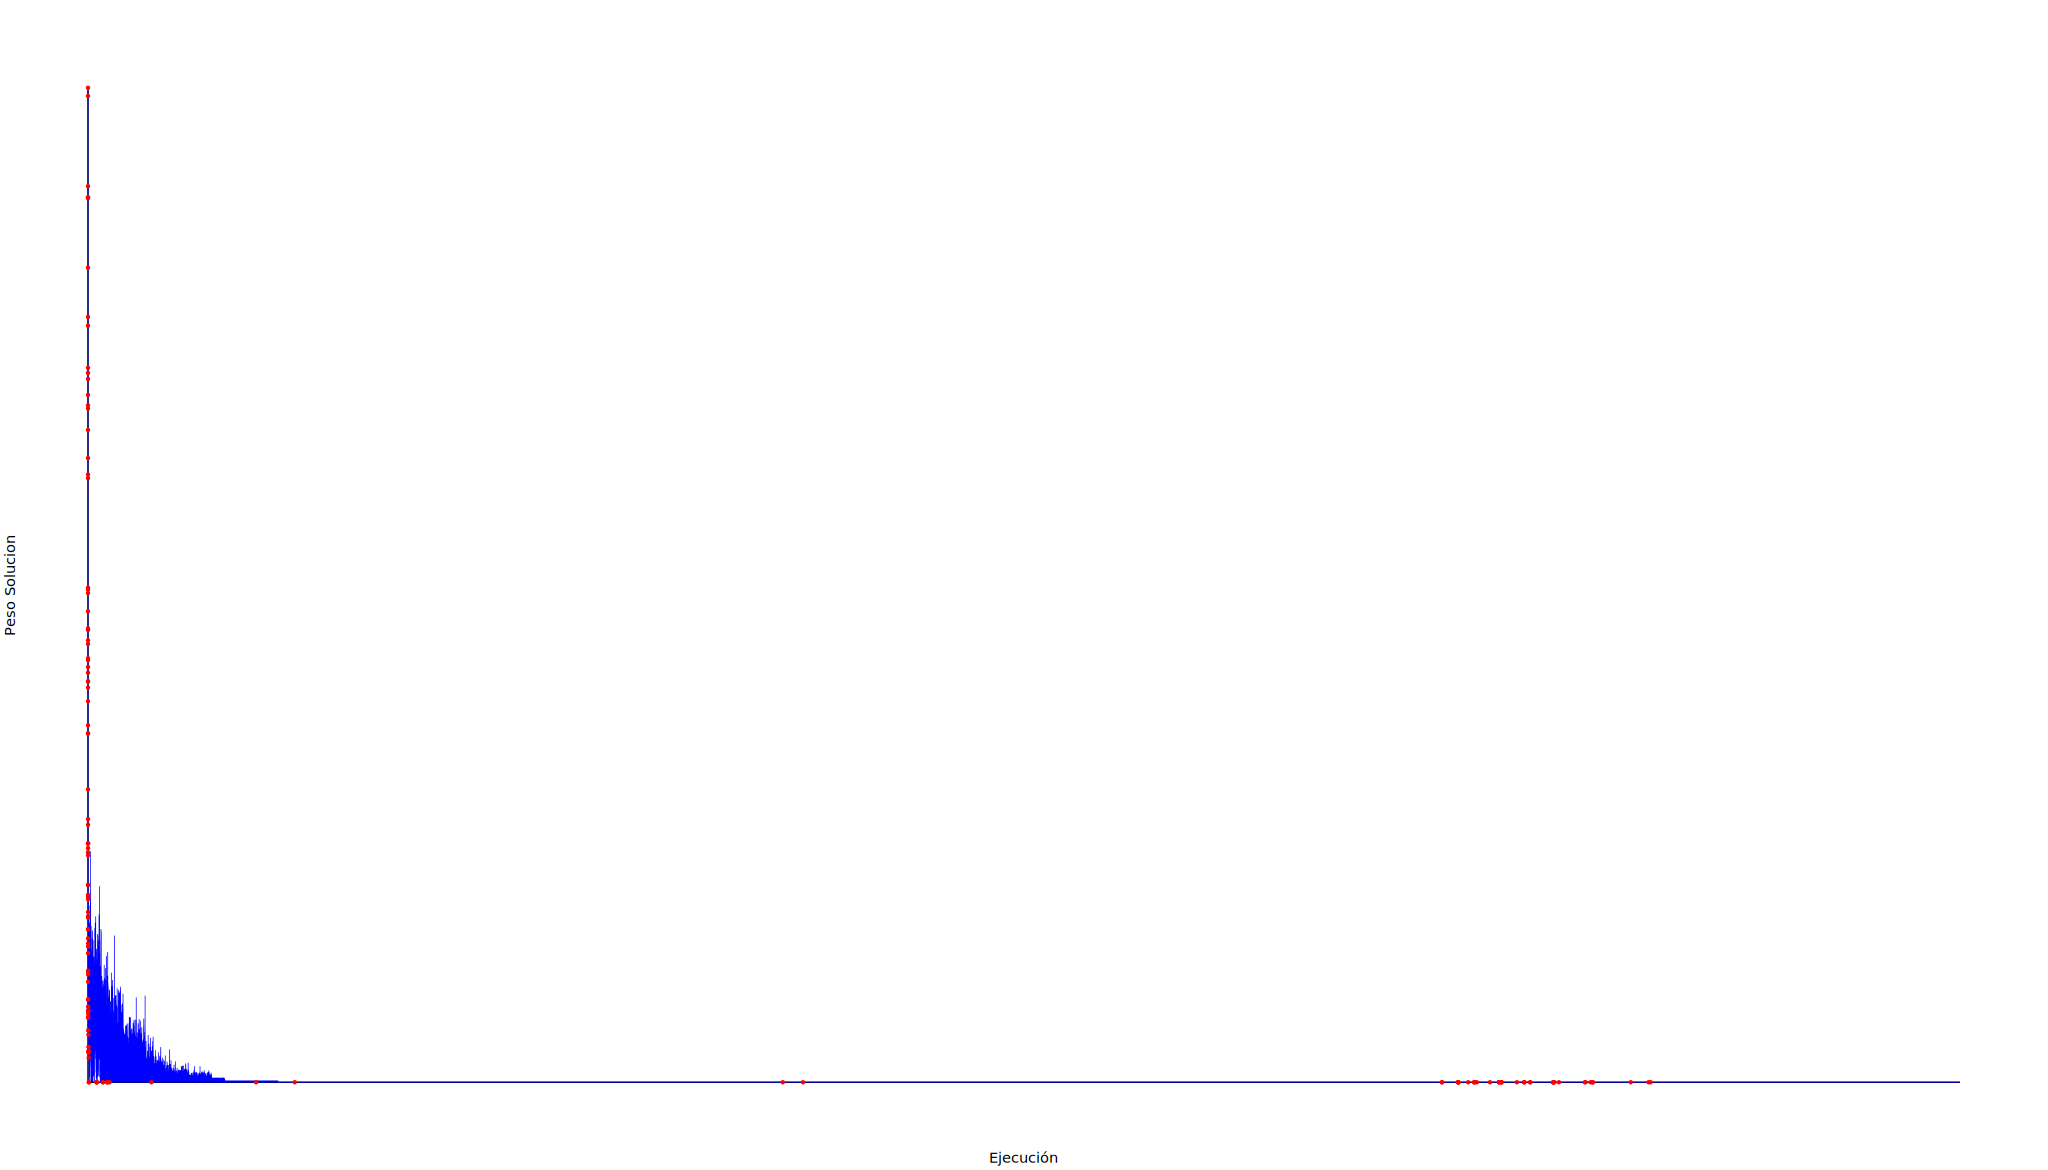
\includegraphics[width=0.4\textwidth]{../svgs/40_documentable_semilla_1.pdf}
    \captionof{figure}{Grafica correspondiente a la primer configuracion}
\end{center}

Siendo que la solucion encontrada corresponde a: $0.3034413264907438$.

Una vez configurado para la instancia de 40 ciudades, se trato con la de 150, obteniendo este resultado: 

\begin{center}
    \includegraphics[width=0.4\textwidth]{../svgs/150_documentable_semilla_82.pdf}
    \captionof{figure}{Grafica correspondiente a la primer configuracion para 150 ciudades}
\end{center}

Siendo que la mejor solución alcanzada en este caso es $0.14021446711368496$ con la semilla 82.

Pero bajar la solución comenzo a volverse cada vez más complicada debido a que los tiempos que toma ejecutar el algoritmo para 15 mil resultados por cada lote es mucho en comparación a otros resultados obtenidos.

Es por ello que lo siguiente es buscar disminuir el numero de lotes generados sin afectar los resultados obtenidos, por lo que la primer manera de intentar realizar esto fue bajar el numero de lotes a 4000 resultados por lote. Pero esto no permitio mejorar mucho los resultados.

Por lo que se probo con la siguiente configuración:

\begin{itemize}
\item \textbf{Temperatura:} 50000
\item \textbf{Lote: } 4000
\item \textbf{$\phi$: } 0.9
\end{itemize}

De esta manera es que la grafica nos queda de la siguiente manera:

\begin{center}
    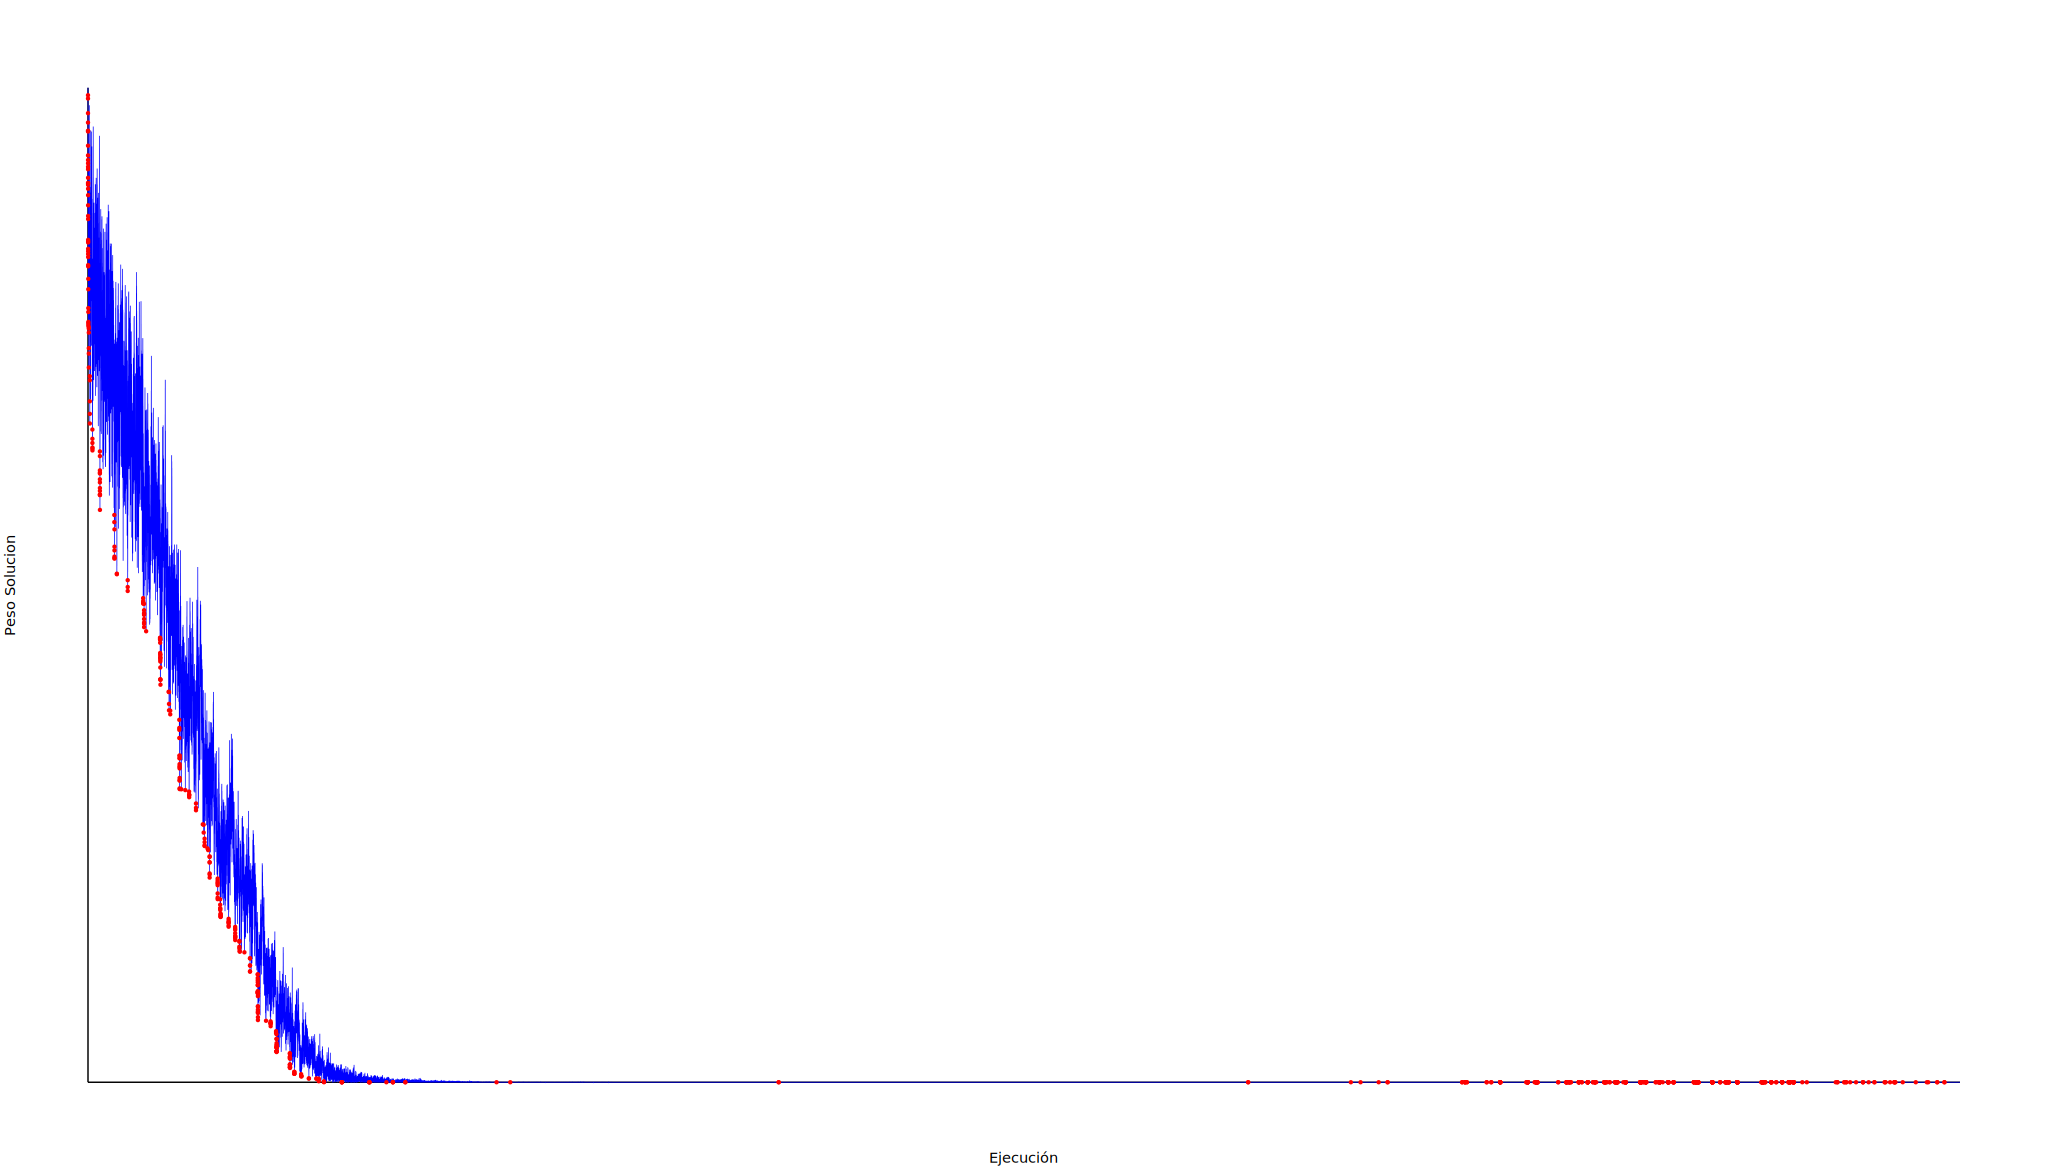
\includegraphics[width=0.4\textwidth]{../svgs/150_documentable_semilla_4.pdf}
    \captionof{figure}{Grafica correspondiente a la segunda configuracion para 150 ciudades}
\end{center}

Siendo que la mejor solución alcanzada en este caso es $0.14351238852956927$ con la semilla 4. Para obtener mejores resultados se necesito de un mayor numero de semillas que las 100 con las que se intento, por lo que se modifico aumentando los lotes.

\begin{itemize}
\item \textbf{Temperatura:} 50000
\item \textbf{Lote: } 6000
\item \textbf{$\phi$: } 0.9
\end{itemize}

De esta manera es que la gráfica resultante nos queda de la siguiente manera:

\begin{center}
    \includegraphics[width=0.4\textwidth]{../svgs/150_documentable_semilla_60.pdf}
    \captionof{figure}{Grafica correspondiente a la tercer configuracion para 150 ciudades}
\end{center}

Siendo que la mejor solución alcanzada en este caso es $0.1494126116684861$ con la semilla 60. De esta forma estamos observando que a pesar de estar aumentando el numero de lotes, esta empeorando la solución obtenida después de hacer el intento con 100 semillas. Siendo de esta manera que después de hacer prueba y error moviendo la temperatura dado que temperaturas muy pequeñas no permiten mejorar los resultados lo suficiente. 

Por lo que, una vez visto esto, se decidió hacer uso de un algoritmo que permita calcular la temperatura basada en el porcentaje de aceptación que queremos para la aceptación en un lote. Haciendo uso de busqueda binaria para el calculo de la temperatura.

Una vez ingresado este, se configuro con el porcentaje de aceptacion a 0.95 y el numero de lotes igual a 6000.

\begin{itemize}
\item \textbf{Temperatura:} 20000
\item \textbf{Lote: } 6000
\item \textbf{$\phi$: } 0.9
\item \textbf{Algoritmo temperatura Lote: } 6000
\item \textbf{Algoritmo temperatura porcentaje: } 0.9
\end{itemize}

De esta manera obtenemos lo siguiente:

\begin{center}
    \includegraphics[width=0.4\textwidth]{../svgs/150_documentable_semilla_99.pdf}
    \captionof{figure}{Grafica correspondiente a la quinta configuracion para 150 ciudades}
\end{center}

Siendo que la mejor solución alcanzada en este caso es $0.14753797072395675$ con la semilla 99. Notamos que los resultados en la gráfica cambiaron, teniendo de esta manera que la figura que surge de la selección de nuestro algoritmo se eleva, dando asi a entender que el algoritmo pierde el tiempo realizando una busqueda en una temperatura demasiado alta.

Por lo que lo siguiente a esto fue disminuir el numero de lotes en el calculo de la temperatura, igualmente disminuir el porcentaje de aceptación. De tal manera que:

\begin{itemize}
\item \textbf{Temperatura:} 20000
\item \textbf{Lote: } 6000
\item \textbf{$\phi$: } 0.9
\item \textbf{Algoritmo temperatura Lote: } 3000
\item \textbf{Algoritmo temperatura porcentaje: } 0.65
\end{itemize}

De esta manera obtenemos lo siguiente:

\begin{center}
    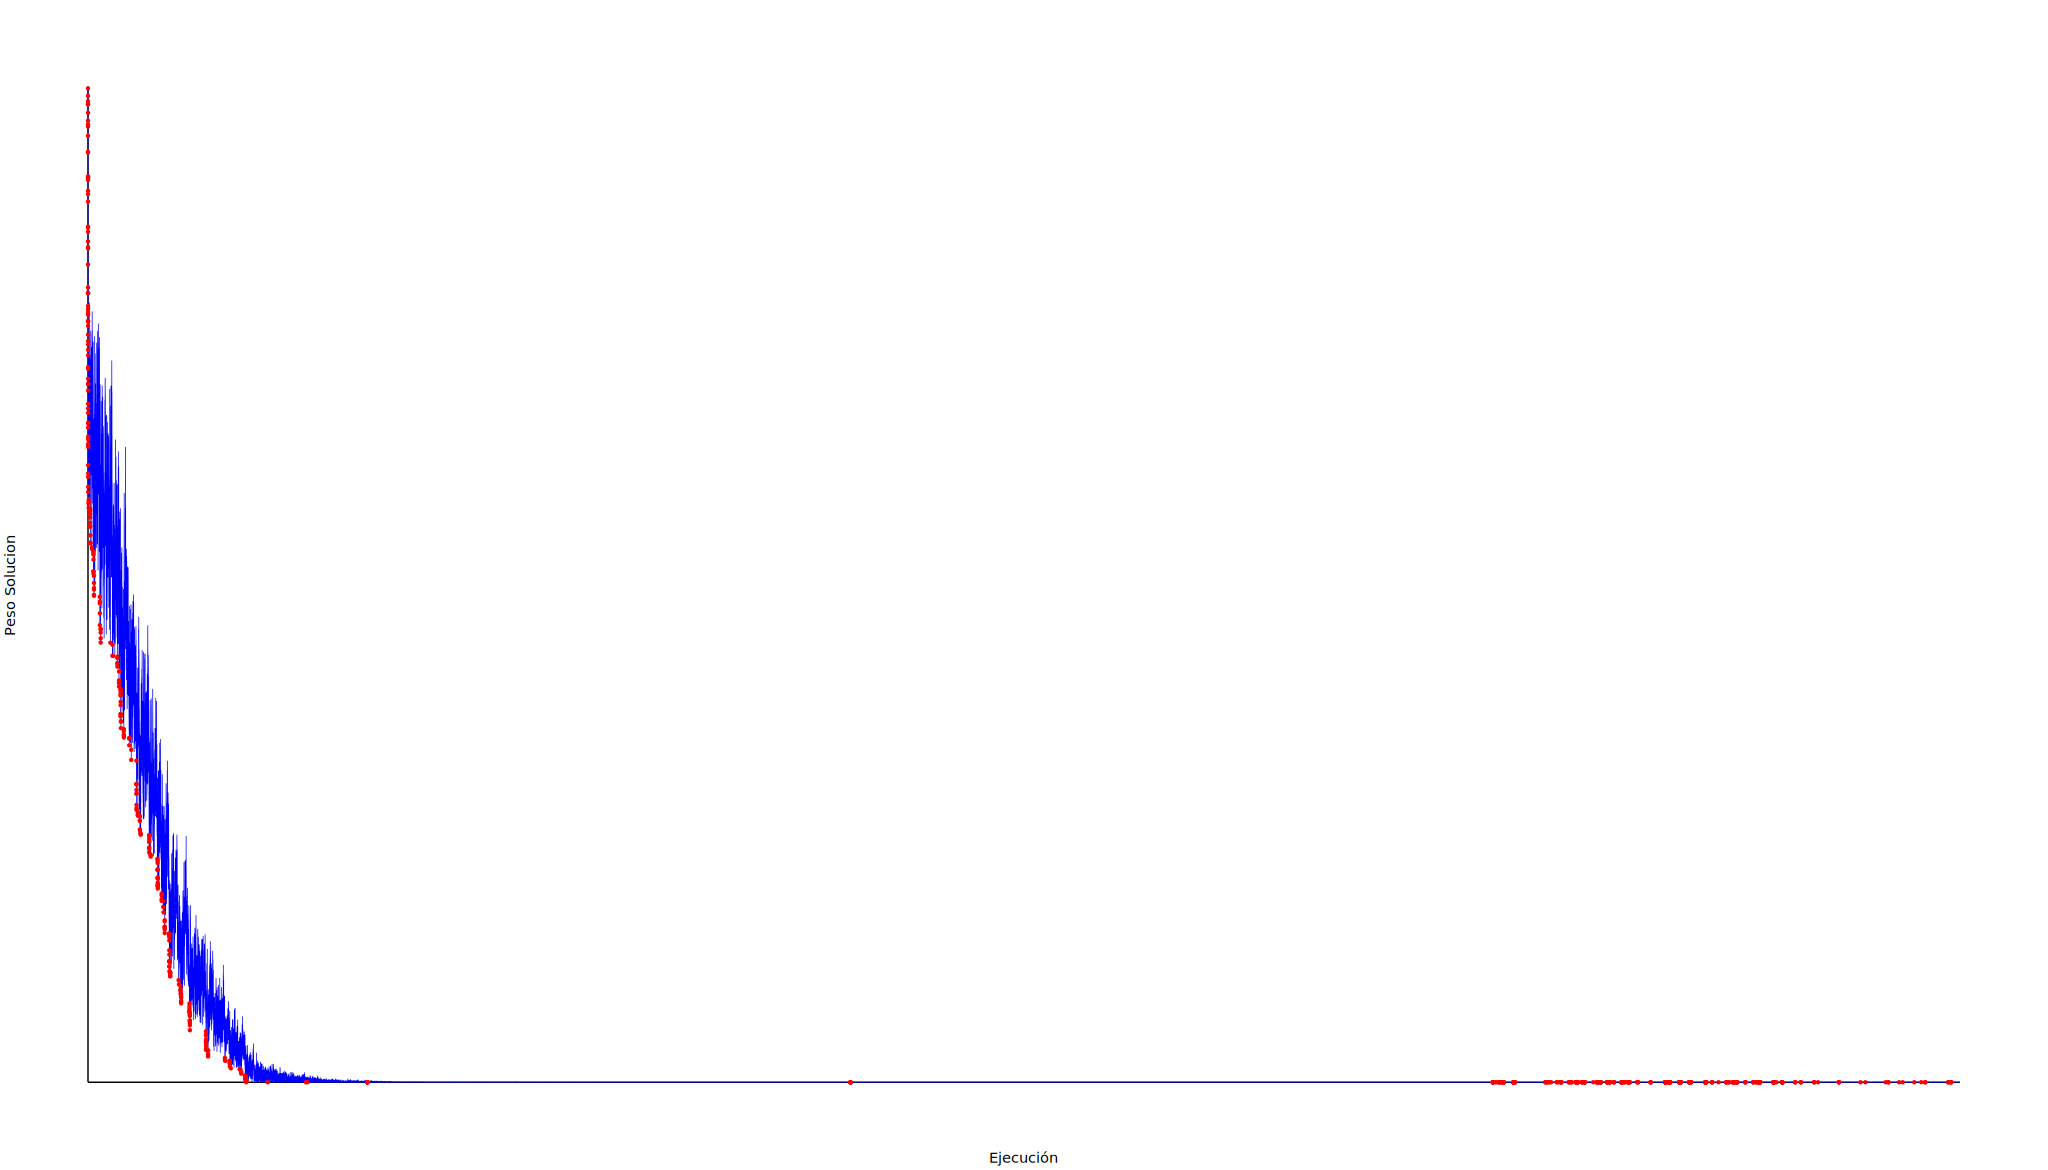
\includegraphics[width=0.4\textwidth]{../svgs/150_documentable_semilla_175.pdf}
    \captionof{figure}{Grafica correspondiente a la sexta configuracion para 150 ciudades}
\end{center}

Siendo que la mejor solución alcanzada en este caso es $0.14756149424092052$ con la semilla 175. Notando de esta manera que la gráfica se aplano, pero aun no podemos conseguir mejorar la solución a pesar de haberlo intentado con 200 semillas. Es por ello que se debe de intentar con mas semillas.

Tratando con mas semillas, podemos encontrar que el mejor resultado obtenido es $0.14122835850399948$, pero aun queremos mejorar los resultados obtenidos.

Para ello debemos de seguir profundizando, por lo que la phi se paso a ser 0.95 para poder seguir profundizando en los resultados.

\begin{itemize}
\item \textbf{Temperatura:} 20000
\item \textbf{Lote: } 6000
\item \textbf{$\phi$: } 0.95
\item \textbf{Algoritmo temperatura Lote: } 3000
\item \textbf{Algoritmo temperatura porcentaje: } 0.65
\end{itemize}

De esta manera obtenemos lo siguiente:

\begin{center}
    \includegraphics[width=0.4\textwidth]{../svgs/150_documentable_semilla_673.pdf}
    \captionof{figure}{Grafica correspondiente a la septima configuracion para 150 ciudades}
\end{center}


Siendo que la mejor solución en este caso es $0.1442443419532619$ con la semilla 143. Pero tratando con mas semillas podemos encontrar que el mejor resultado obtenido es $0.14148027872431046$ con la semilla 673.

Pero seguimos esperando mejorar los resultados, dado que la aleatoriedad forma parte del algoritmo, entre mejor sea la semilla, mejor será el resultado obtenido, de ahi que podemos seguir tratando con distintas semillas y veremos que el resultado mejora. Pero antes de eso buscamos una configuración que inclusive mejore:

\begin{itemize}
\item \textbf{Temperatura:} 20000
\item \textbf{Lote: } 7000
\item \textbf{$\phi$: } 0.95
\item \textbf{Algoritmo temperatura Lote: } 3500
\item \textbf{Algoritmo temperatura porcentaje: } 0.60
\end{itemize}

De esta manera obtenemos lo siguiente:

\begin{center}
    \includegraphics[width=0.4\textwidth]{../svgs/150_documentable_semilla_118.pdf}
    \captionof{figure}{Grafica correspondiente a la octava configuracion para 150 ciudades}
\end{center}

Siendo que la mejor solución obtenida en este caso es $0.14002260979550915$ con la semilla 118. Pero al realizar mas intentos haciendo uso de distintas semillas, es que he podido llegar a $0.13779347989236584$ con la semilla -182984. 

De esta manera obtenemos lo siguiente:

\begin{center}
  \includegraphics[width=0.4\textwidth]{../svgs/Mejor_150_semilla_-182984.pdf}
  \captionof{figure}{Grafica correspondiente a la novena configuracion para 150 ciudades}
\end{center}

Finalmente es que podemos llegar a la mejor solución que he encontrado hasta el momento, la cual es $0.13667417380708738$ de la semilla -244383  

\begin{center}
  \includegraphics[width=0.4\textwidth]{../svgs/Mejor_150_semilla_-244383.pdf}
  \captionof{figure}{Grafica correspondiente a la novena configuracion para 150 ciudades}
\end{center}


\section{Conclusión y Trabajos Futuros}

De esta manera es que podemos mostrar la mejor solución encontrada, la cual después de nuestras configuraciones y ejecuciones con distintas semillas es que podemos ver que nuestro mejor resultado está dado por $0.13667417380708738$. Notando a lo largo del desarrollo y de los resultados es que podemos encontrarnos la importancia de la temperatura optima dada la semnilla a evaluar.

Mientras que a mayor lotes es más facil obtener buenos resultados, pero es dificil profundizar en esos valores debido a que termina saltando de un lado a otro contantemente el algoritmo. Por otro lado a lotes demasiado pequeños no explora lo suficiente y no alcanza a profundizar con suficiente eficiencia.

Inclusive al realizar una buena implementación del algoritmo y una buena configuración que consiga buenos resultados, los mejores resultados es como encontrar una aguja en un pajar, debido a que incluso los resultados que bajan de $.14$ son resultados bastante ocasionales, mientras que los que rompan ese limite cada vez con mejores resultados son inclusive más imposibles de obtener.

Por lo que es importante elegir un correcto numero de lotes, una temperatura que se adecue a esa cantidad de lotes esto debido a que esta muy relacionados el tamaño de lote con la temperatura que usa la heuristica. Finalmente a mayor $\phi$ es que podemos dar mayor oportunidad de profundizar los resultados.

Concluyendo de esta manera que nuestra mejor configuración alcanzada está dada por:

\begin{itemize}
\item \textbf{Temperatura:} 20000
\item \textbf{Lote: } 7000
\item \textbf{$\phi$: } 0.95
\item \textbf{Algoritmo temperatura Lote: } 3500
\item \textbf{Algoritmo temperatura porcentaje: } 0.60
\end{itemize}

y la mejor solución alcanzada esta dada por $0.13667417380708738$ y la cual es la siguiente [171, 652, 1075, 483, 512, 821, 75, 346, 183, 179, 671, 16, 520, 186, 675, 340, 502, 1038, 12, 828, 151, 339, 826, 444, 17, 25, 492, 491, 499, 347, 817, 489, 4, 174, 165, 3, 333, 27, 353, 990, 981, 988, 23, 176, 668, 352, 978, 5, 6, 1004, 351, 991, 185, 22, 213, 676, 163, 172, 182, 496, 19, 839, 815, 184, 667, 656, 507, 7, 823, 678, 816, 187, 982, 14, 181, 332, 345, 820, 26, 654, 490, 653, 344, 665, 673, 173, 2, 9, 1, 829, 661, 832, 663, 657, 508, 986, 505, 168, 329, 509, 493, 979, 837, 995, 984, 501, 164, 11, 1003, 349, 331, 662, 8, 999, 334, 674, 985, 343, 510, 660, 20, 825, 500, 504, 511, 327, 670, 350, 840, 336, 980, 297, 1001, 74, 822, 166, 658, 666, 818, 655, 819, 330, 1073, 169, 1037, 326, 328, 167, 495, 494]

Mientras que para la de 40 instancias está dado por $0.3034413264907438$ donde la permutación es la siguiente: [1, 815, 653, 490, 654, 816, 2, 163, 329, 493, 979, 4, 165, 3, 981, 978, 817, 489, 492, 491, 164, 327, 980, 74, 166, 658, 666, 818, 655, 819, 330, 1073, 169, 1037, 814, 326, 328, 167, 495, 494] 

\begin{thebibliography}{99}

\bibitem{una-referencia} Peláez V. C.(2025). El Problema del Agente
Viajero [Material de clase]. Universidad Nacional Autónoma de México, Ciudad de México.

\bibitem{una-referencia} Peláez V. C.(2025). Aceptación por Umbrales [Material de clase]. Universidad Nacional Autónoma de México, Ciudad de México.

\end{thebibliography}


\end{multicols}

\end{document}
